\documentclass[a4paper, 12pt]{article}
\usepackage[utf8x]{inputenc}
\usepackage{cmap}
\usepackage[english, russian]{babel}
\usepackage{indentfirst}
\usepackage[left=20mm, top=20mm, right=20mm, bottom=20mm]{geometry}
\usepackage{tikz}
\usepackage{float}
\usepackage{amsmath, amsfonts, amssymb}
\usepackage{graphicx}
\usepackage{fancybox, fancyhdr}
\usepackage{hyperref}
\usepackage{listings}
\usepackage{caption}
\usepackage{subcaption}
\usepackage{xcolor}
\usepackage{paralist}
\pagestyle{fancy}
\fancyhf{}
\fancyhead[L]{Лабораторная работа №7}
\fancyhead[R]{Линейные системы автоматического управления}
\fancyfoot[C]{\thepage}
\graphicspath{{images/}}
\usetikzlibrary{patterns}
\definecolor{LightGray}{gray}{0.95}
\definecolor{LightGray2}{gray}{0.7}
\hypersetup{
    colorlinks=true,
    linkcolor=blue,
    filecolor=magenta,
    urlcolor=cyan,
    pdftitle={contents setup},
    pdfpagemode=FullScreen,
}
\setlength{\parskip}{1.5mm}
\setlength{\headheight}{15pt}
\setlength{\footskip}{15pt}
\allowdisplaybreaks

\begin{document}
    \begin{titlepage}

        \begin{center}
        
\includegraphics[width=0.3\textwidth]{itmo.png} % requires itmo.png in /images folder
        \vfill
        
        Федеральное государственное автономное образовательное учреждение высшего образования
        «Национальный Исследовательский Университет ИТМО»\\
        
        \vfill
        {\large\bf ЛАБОРАТОРНАЯ РАБОТА №6}\\
        {\large\bf ПРЕДМЕТ «ЛИНЕЙНЫЕ СИСТЕМЫ АВТОМАТИЧЕСКОГО УПРАВЛЕНИЯ»}\\
        {\large\bf ТЕМА «АНАЛИЗ ТОЧНОСТИ СИСТЕМ УПРАВЛЕНИЯ»}\\
        Вариант 4
        \vfill

        \begin{flushright}
            \begin{minipage}{.45\textwidth}
            {
                \hbox{Преподаватель: Золотаревич В. П.}
                \hbox{Студент: Румянцев А. А.}
                \hbox{Поток: ЛСАУ R22 бак 4.1.1}
                \hbox{}
                \hbox{Факультет: СУиР}
                \hbox{Группа: R3341}
            }
            \end{minipage}
        \end{flushright}
        
        \vfill
                
        Санкт-Петербург\\
        2024
        \end{center}
    \end{titlepage}
    
    \tableofcontents

    \newpage
    \section{Цель работы}
    Исследование точностных свойств систем управления.


    \section{Задание 1}
    \subsection{Условие}
    \textit{Исследование системы с астатизмом нулевого порядка.}
    \begin{compactitem}
        \item Структура системы представлена на рис. \ref{fig:struct_scheme1}, где $H(s)=k$. Передаточная функции объекта
        управления $$W(s)=\dfrac{1.5}{s^2+2s+1},$$ характеристики задающего воздействия $g(t):1,t$
        \begin{figure}[H]
            \centering
            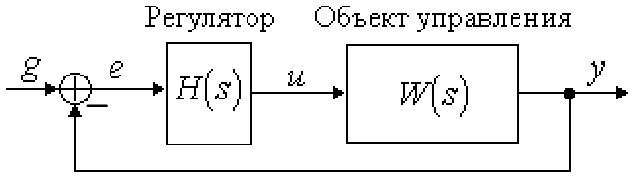
\includegraphics[scale=0.7]{struct_scheme1.png}
            \captionsetup{skip=0pt}
            \caption{Схема эксперимента}
            \label{fig:struct_scheme1}
        \end{figure}
        \item Исследование стационарного режима работы: $g(t)=A$.
        Получить переходные процессы для трех различных значений
        коэффициента $k$ и определить предельное
        значение установившейся ошибки $\varepsilon$.
        Значения коэффициента $k$ (здесь и во
        всех последующих пунктах): $1, 5, 10$.
        \item Исследование режима движения
        с постоянной скоростью: $g(t)=Vt$.
        Получить переходные процессы для различных
        значений коэффициента $k$. Интервал наблюдения --
        $30$ секунд.
    \end{compactitem}
     

    \subsection{Выполнение}


    \section{Задание 2}
    \subsection{Условие}
    \textit{Исследование системы с астатизмом первого порядка.}
    \begin{compactitem}
    \item Структура системы представлена на рис. \ref{fig:struct_scheme1}, где
    $H(s)=k/s$. Передаточная функция объекта управления $$W(s)=\dfrac{s+1.5}{s^2+2s+1},$$
    характеристики квадратично нарастающего задающего воздействия $$g(t)=\dfrac{at^2}{2}=0.4t^2$$
    Характеристики постоянного и линейно нарастающего задающих воздействий взять из задания 1.
    \item Исследование стационарного режима работы: $g(t)=A$.
    Получить переходные процессы для различных значений коэффициента $k$ и определить предельное
    значение установившейся ошибки $\varepsilon$.
    \item Исследование режима движения с постоянной скоростью: $g(t)=Vt$.
    Получить переходные процессы для различных значений коэффициента $k$ и определить
    предельное значение установившейся ошибки $\varepsilon$. Интервал наблюдения -- $30$ секунд.
    \item Исследование режима движения с постоянным ускорением: $g(t)=at^2/2$.
    Получить переходные процессы для различных значений коэффициента $k$. Интервал
    наблюдения -- $30$ секунд.
    \end{compactitem}


    \subsection{Выполнение}


    \section{Задание 3}
    \subsection{Условие}
    \textit{Исследование влияния внешних возмущений.}
    \begin{compactitem}
        \item Cобрать схему моделирования возмущенной системы. Дано:
        $$W(s)=\dfrac{1.5}{s^2+2s+1},\ \ f_1(t)=2,\ \ f_2(t)=1$$
        Структура системы представлена на рис. \ref{fig:struct_scheme3}.
        \begin{figure}[H]
            \centering
            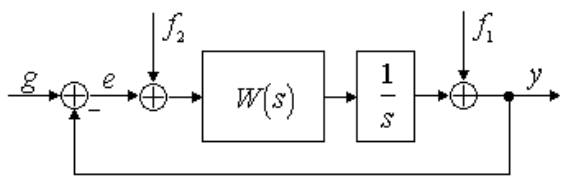
\includegraphics[scale=0.75]{struct_scheme3.png}
            \captionsetup{skip=0pt}
            \caption{Схема эксперимента}
            \label{fig:struct_scheme3}
        \end{figure}
        \item Полагая $f_2(t)\equiv0$ и $g(t)=1(t)$, получить переходной процесс и определить
        предельное значение установившейся ошибки $\varepsilon$.
        \item Полагая $f_1(t)\equiv0$ и $g(t)=1(t)$, получить переходной процесс и определить
        предельное значение установившейся ошибки $\varepsilon$.
    \end{compactitem}


    \subsection{Выполнение}


    \section{Задание 4}
    \subsection{Условие}
    \textit{Исследование установившейся ошибки при произвольном входном воздействии.}
    Структура системы представлена на рис. \ref{fig:struct_scheme1}, где $H(s)=1$. Дано:
    $$W(s)=\dfrac{1.5}{s^2+2s+1},\ \ g(t)=0.4t+0.2t^2$$
    \begin{compactitem}
    \item Получить переходной процесс в замкнутой системе
    и определить (по графику) установившуюся ошибку слежения $e_y(t)$.
    \item Получить приближенное аналитическое выражение для $e_y(t)$, сохранив в
    ряде Тейлора $$e_y(t)=c_0g(t)+c_1\dfrac{d}{dt}g(t)+\dfrac{c^2}{2!}\dfrac{d^2}{dt^2}g(t)+\dfrac{c^3}{3!}\dfrac{d^3}{dt^3}g(t)...,$$
    где $c_i$ -- коэффициенты ошибок, три первых члена. Построить график $e_y(t)$
    в соответствии с полученным аналитическим выражением (использовать для этого блок нелинейных функций Fnc).
    \end{compactitem}


    \subsection{Выполнение}
\end{document}